\section{Reformulation: a learning approach }
\label{mlreformulation}

Efficiency of neural network nowadays can be very good. An approach based on network is also used here. But, the aim is not to learn answering question. There are two reasons for that. First the knowledge changes over time, e.g. the president name depends on the date. Then, something simple is wished. The learning process should also not be continuous. Learning the answer implies to know proper Names which increase the size of the dictionary, that means increasing the learning time. 

The module presented here tries to reformulate a question. In fact it tries to translate the question for the wikidata module. It means adapting it as most as possible for this module, correct the mistakes of grammatical parsing, as it is illustrated in figure \ref{figexmlrefref}.

\begin{figure}
    \centering
  \begin{tikzpicture}
  \node (10) at (8,11.5) {\textsc{When was the president of the United States born?}};
  \node (0) at (10,10) {$\triple$};
  \node[color=mLightBrown] (1) at (10,8.5) {president};
  \node (2) at (12,8.5) {?};
  \node (3) at (8,8.5) {$\triple$};
  \node (4) at (8,7) {United States};
  \node[color=mLightBrown] (5) at (5,7) {birth date};
  \node (6) at (10,7) {?};

  \draw[->, >=latex] (0) edge node[sloped, anchor=center, above] {\scriptsize{pred.}} (1);
  \draw[->, >=latex] (0) edge node[sloped, anchor=center, above] {\scriptsize{obj.}} (2);
  \draw[->, >=latex] (0) edge node[sloped, anchor=center, above] {\scriptsize{subj.}} (3);
  \draw[->, >=latex] (3) edge node[sloped, anchor=center, above] {\scriptsize{subj.}} (5);
  \draw[->, >=latex] (3) edge node[sloped, anchor=center, above] {\scriptsize{obj.}} (6);
  \draw[->, >=latex] (3) edge node[sloped, anchor=center, above] {\scriptsize{pred.}} (4);
  \draw[<->, >= latex,color=mLightBrown] [draw=mLightBrown] [bend right=50, above] (1) edge (5);
  
 \end{tikzpicture}
 \caption{An example of bad triple formation, ``president'' and ``United States'' terms are in the wrong place. The reformulation module should solve this kind of problem.}
\label{figexmlrefref}
\end{figure}

\subsection{How it works}


The grammatical module builds a tree representation of the question. The reformulation module work on this output, so with a tree representation. The assumption ``all useful information is kept in this form''  is also necessary. The module has also a dictionary. There are four steps to do. First a pretreatment replace proper names and numbers with tags, such that all words of the triple are in the dictionary, then the request is projected in the math space of request. Two last steps reveres the two first, but the reverse projection should produce a better request, which mean the final request is adapted for the Wikidata module.

For compatibilities reasons, we do not work with the actual data model which is too complicated. In fact we need a regular triple representation, that means all operators must be transformed, this step is easy. For unitary operators, $O(f)$ becomes $(f,O,?)$; for binary operators, $aOb$ becomes $(a,O,b)$. This operation does not weak the expressive power.

\subsubsection{Mathematical spaces}

The mathematical space of request $\mathcal{R}$ is simply the subset of the $\mathbb{R}$ vector space of dimension 50, were all vector have a Euclidean norm of 1.
A triple is formed of a subject request, a predicate and an object request, it is also natural to consider the triple over $\mathcal{R}$, which elements order with always be subject, predicate, object.
Let us call vector the elements of $\mathcal{R}$.

The choice of a 50-dimension can be modified if necessary, but taking a higher dimension could slow the learning process, and with a lower space we could lose some expressive power, which may lead to very poor results.

%To unify everything As we works with requests, we consider everything is a request, even a word.

%There are 2 generic spaces: the one of words which is a vector space of dimension 50 and the space of request which is the space of word triples. The first word of a triple represents the subject, the second represents the predicate and the last the object.
%To distinguish words which are vectors and words with letters, we will add the adjective English to the seconds.

\subsubsection{Dictionary}

The dictionary defines matching between English words and vectors triple, which is the base of the process. We use triple because a word could have different meaning depending on his nature, so predicate vector for a word is not the same as subject vector which is not the same as object vector. We will denote m.s subject vector of word m, m.p and m.o for predicate and object.

\subsubsection{Pre- and post-treatment and treatment}

We evoke some reasons not to handle proper name directly (the dictionary size would increase and names could change), there is another argument: there is an arbitrary number of proper names, because you can invent some new names every time. That is why they are replaced in a request by a tag NAMEi, $i\in{1,2,3}$. It allows us to have three different names in a question, and that is sufficient. The same happens to the numbers. Tag UNKNOWN finally represents the ``holes'' in the request tree. At the end, after the treatment we replace tags with corresponding real names or numbers in the final tree.

Recognizing a number is not hard, in fact it is just checking it the character sequence looks like numbers optionally followed by a dot and numbers. If the sequence is not a number or a ``hole'' and is not in the dictionary, the module treats it as a proper name.

\subsubsection{Project form a request to a vector}

The model allows an arbitrary request form, it means we have a tree with an unknown depth, and to keep the complete question information we should handle it so. But the request are triple, so it is easy to transform. First with the dictionary all words are replaced with vectors, of course we take the vector corresponding to the function of the word in the tree. Then we have to ascend the whole tree to compute the root value.

Let define a matrix compact which takes a triple of vector and merge them in one vector, here merging in not an intuitive operation, in fact we don't know how to merge this triple, that is why all coefficients of the matrix are unknown. To compute what we call a vector, output should be normalized.

Now by applying this operation bottom-up in the tree. The main idea is each node value represent the subtree request.

\begin{figure}
\begin{center}
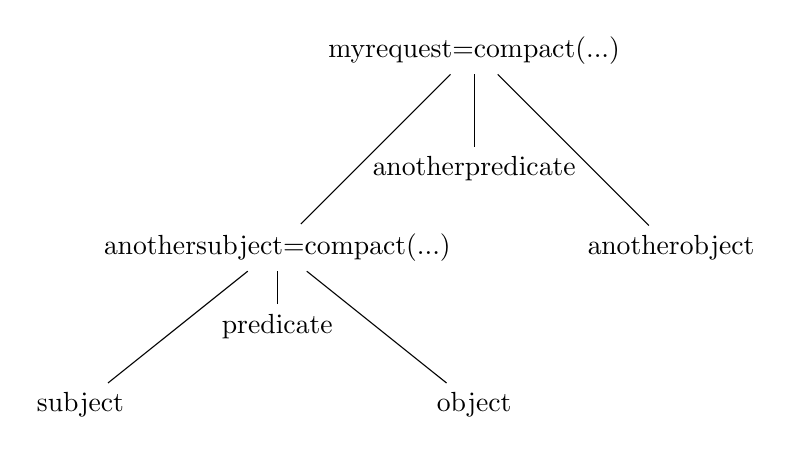
\begin{tikzpicture}[x=2.5cm]
\node (s) at (1,0) {subject};
\node (p) at (3,0) {object};
\node (r) at (2,1) {predicate};


\node (a) at (2,2) {anothersubject=compact(...)};
\node (b) at (4,2) {anotherobject};
\node (l) at (3,3) {anotherpredicate};
\node (h) at (3,4.5) {myrequest=compact(...)};

\draw (s)--(a)--(p);
\draw (r)--(a);
\draw (a)--(h)--(b);
\draw (l)--(h);
\end{tikzpicture}
\caption{The process of projection, an example}
\end{center}
\end{figure}

\subsubsection{Reconstruct a request from a vector}

This operation is quite symmetrical of the projection, with a matrix uncompact we can the same way obtain a vector triple from a vector, and recursively a tree appear. But the question is how to know if we should reapply the function uncompact or leave the vector as a leaf? First say in a triple predicate is never a tree, then object and subject will be let as leaf if a known word is near enough. Finally each node is replaced with the nearest corresponding word in the dictionary, that mean, for example, for a vector in middle of a triple which is also a predicate, take word with nearest predicates' vector.

Defining near enough is difficult. To avoid infinite loop we will take depth of nodes into account. We must take $\delta>0$ a precision factor and $g$ a growth factor. If $d$ is the depth of node $n$, near enough means distance is bounded by $\delta*g^d$ with regard of Euclidean norm.  

\begin{figure}
\begin{center}
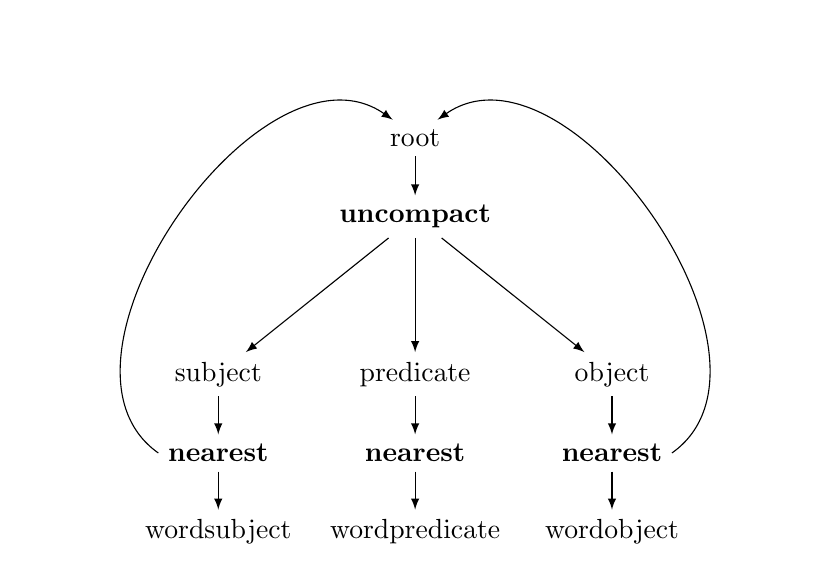
\begin{tikzpicture}[x=2.5cm]
\node (s) at (1,0) {subject};
\node (p) at (3,0) {object};
\node (r) at (2,0) {predicate};
\node (sf) at (1,-1) {\textbf{nearest}};
\node (pf) at (3,-1) {\textbf{nearest}};
\node (rf) at (2,-1) {\textbf{nearest}};
\node (sw) at (1,-2) {wordsubject};
\node (pw) at (3,-2) {wordobject};
\node (rw) at (2,-2) {wordpredicate};
\node[rectangle] (b) at (2,2) {\textbf{uncompact}};
\node (v) at (2,3) {root};
%\node (b) at (4,2) {b};
%\node (l) at (3,3) {l};
%\node (h) at (3,4) {h=compact(a,l,b)};

\draw[->, >=latex] (b)--(s);
\draw[->, >=latex] (b)--(p);
\draw[->, >=latex] (b)--(r);
\draw[->, >=latex] (v)--(b); % WTF?
\draw[->, >=latex] (r)--(rf);
\draw[->, >=latex] (p)--(pf);
\draw[->, >=latex] (s)--(sf);
\draw[->, >=latex] (rf)--(rw);
\draw[->, >=latex] (pf)--(pw);
\draw[->, >=latex] (sf)--(sw);

\draw [->, >=latex] (pf.east)        to [bend right=90] (v);
\draw [->, >=latex] (sf.west)        to [bend left=90] (v);
\end{tikzpicture}
\caption{The algorithm \textsc{reconstruction} in a scheme}
\end{center}
\end{figure}

The algorithm reconstruct is also:



\begin{algorithm}[H]
    \DontPrintSemicolon  % Some LaTeX compilers require you to use \dontprintsemicolon instead
    \KwIn{$\delta>0$ and $a\in A$}
    \KwOut{request tree}
    $(s,p,o) \gets \text{uncompact}(a)$\;
    Find m s.t. $\N{m.s-s}<\delta$ is minimal \;
    \lIf{m exists}{
        $s \gets m$
    }
    \lElse{
        $s \gets reconstruct(\delta*g,s)$
    } 
    Find m s.t. $\N{m.o-o}<\delta$ is minimal \;
    \lIf{m exists}{
        $o \gets m$
    }
    \lElse{
        $o \gets reconstruct(\delta*g,o)$
    } 
    $p \gets {\text{argmin}}_m  (\N{m.p-p})$\;
    \Return{$(s,r,o)$}\;
    \caption{\textsc{reconstruct} From vector to tree}
\end{algorithm}

\subsubsection{Remarks}

Matrix compact and uncompact are not bijective after restraining the request space to existent requests. Applying uncompact then compact should give the identity, with of course an error margin, but when compacting then uncompacting we only have to find an equivalent request, i.e. with the same meaning but with another formulation. If it were not the case it would produce exactly the same output as the input, that would be useless.

\subsection{Learning}

Training the model cannot be done easily with a classic back-propagation because we have no idea what is the best triple for a question. The solution is also to try to change a little the matrix, and see what changes improve the better the quality of result, it is however very bad in cost. 

Now to compute the quality of the result, i.e. the score  of the module we use a semantic distance: it's a norm depending on the meaning of words. To be simple we base it of the relation graph ``instance of'' of Wikidata assuming it is a directed acyclic graph. We compute the nearest common ancestor and we add the distance between this node and the two word  nodes.

\subsection{Implementation}

The module is written in C++, with threads to speed up the matrix multiplication. To interface it with the others, it is built as a shared library with python library. The dictionary has been generated using the clex \footnote{\url{https://github.com/Attempto/Clex}}. 

\subsection{Future work}

The learning process has not been made yet. As latency with Wikidata is very high (several seconds) we have to download Wikidata and run it in local.

Then we could think of different manners to train the model.

At least we could think about a good manner to find the nearest word in the dictionary. It can be done with a linear time, but considering there are 100 000 words in the dictionary, cost is not negligible. As we work in dimension 50, it is not a trivial problem to find an efficient method to obtain a logarithmic complexity. Kd-trees allow a search in log-time (with preprocessing); but with dimension 50, the constant factor $2^{50}$ is too large. One line of research were to use distance sensitive hash.

%Finding a way to learn everything with first or second approach is the most important, as the first answering module in functional, learning is possible. Then, learning and computation speed-up will be important, the search for nearest neighbor is long, maybe it is linear, but with near 100 000 words and high dimension it becomes consequent, use of heuristics could be a good idea, for example there exists distance sensitive hash.

